\documentclass[10pt,xcolor=dvipsnames]{beamer}

\usetheme{Frankfurt}
%\usetheme{Bergen}
%\usetheme{Goettingen}
\usepackage{listings}
\usepackage{paralist}
\usecolortheme[RGB={0,104,139}]{structure}%deepskyblue
%\usecolortheme[named=Maroon]{structure}

\title[Cloud based IT Infra with Central Identity]{Cloud based IT Infra with Central Identity}
\subtitle{Final Presentation}

\author{ \underline{Project Guide} \\ \hspace{2mm} \\ \small{ T. Chandra Shekar } \tiny \\ \underline{} \\ \scriptsize \textit{Lecturer -- Dept. of CSE} }
\institute{ \underline{Presenting by} \\ \hspace{2mm} \\ \textit {Team r3b00+ }  \\ \hspace{4mm} \\ Dept. of CSE, RGUKT -- Nuzvid}
\usepackage{color}
 
\definecolor{codegreen}{rgb}{0,0.6,0}
\definecolor{codegray}{rgb}{0.5,0.5,0.5}
\definecolor{codepurple}{rgb}{0.58,0,0.82}
\definecolor{backcolour}{rgb}{0.95,0.95,0.92}
\lstdefinestyle{mystyle}{
    backgroundcolor=\color{backcolour},   
    commentstyle=\color{codegreen},
    keywordstyle=\color{magenta},
    numberstyle=\tiny\color{codegray},
    stringstyle=\color{codepurple},
    basicstyle=\footnotesize,
    breakatwhitespace=false,         
    breaklines=true,                 
    captionpos=b,                    
    keepspaces=true,                 
    numbers=left,                    
    numbersep=5pt,                  
    showspaces=false,                
    showstringspaces=false,
    showtabs=false,                  
    tabsize=2
}
 
\lstset{style=mystyle}

\AtBeginSection[]
{
	\begin{frame}
		\frametitle{Outline}
		\tableofcontents[currentsection,hideothersubsections]
	\end{frame}
}
%\AtBeginSubsection[] % Do nothing for \subsection*
%{
%\begin{frame}<beamer>
%\frametitle{Outline}
%\tableofcontents[currentsection,]
%\end{frame}
%}

\begin{document}


\begin{frame}
\titlepage
\end{frame}

%\begin{frame}
%\frametitle{Outline}
%\tableofcontents[hideallsubsections]
%\end{frame}

\begin{frame}{About us}

\small
\begin{center}
We are from team \textit{r3b00+}  \{reboot\} \\ \hspace{4cm} \\
\begin{tabular}{l  l }
T. Aneesh Kumar & N090247   \\
P. Nageswarao  & N091030  \\
P. Anesh  & N090977 \\
P. Jyothi Ram & N090990 \\
K. Naresh Chowdary  & N090331 \\
N. Venkata Sateesh  & N090935 \\
M. Sanyasirao & N090891  
\end{tabular}


\end{center}


\end{frame}
 

\section{Objective}
\subsection{Objective}
\begin{frame}{Objective}

Our objective is to create a  private cloud and availing access of all its services using central identity with single sign on through dynamic role based management along with REST API to third party for application developers and users. \newline

This can be developed by using open source tools like OpenStack, NFS, LDAP, Ubuntu and etc \newline

Expecting to serve with virtual machines to the research, virtual labs rather than dedicated lab hardware.
\end{frame}

\subsection{Motivation}
\begin{frame}{Motivation}

\begin{itemize}
	\item No Central Identity, Central Storage \& High capacity hardware resource pool.
	\item Failed to maintain large user load web services like ONB, Exam servers, etc.
	\item Dedicated computer course labs like Matlab, VLSI, etc.
	\item No proper Web Application Security \& Standards.
	\item Inadequate resource requirements for Research.
\end{itemize}

\end{frame}



\section{Proposed System}
\subsection{Users \& IT Services}
\begin{frame}{Users \& IT Services}
We are collaborating all IT Services that are required for University and identifing the users who is going to use them. All Users are catagorized into 4 groups $ ^{[1]}$
	
	\begin{itemize}
	\item Studens, Developers, Staff, faculty \& Researches
	\end{itemize}
\begin{figure}[H]
\begin{center}
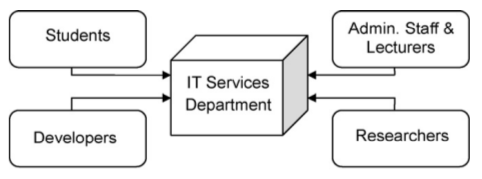
\includegraphics[width=5cm]{./it.png}
\caption{ Simplified structure of the main users of IT services. \label{fig:Simplified structure of the main users of IT services. }}
\end{center}
\end{figure}
	
\end{frame}
\subsection{Cloud Infrastructures}
\begin{frame}{Cloud Infrastructures}
All University IT Services are deployed in a private cloud, constructed over exsiting infrastructure, that can be broadly viewed as 
	
\begin{figure}[H]
\begin{center}
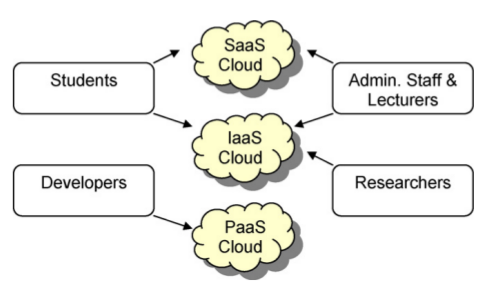
\includegraphics[width=7cm]{./it2.png}
\caption{ IT Services and Users in Cloud Computing\label{fig:IT Services and Users in Cloud Computing }}
\end{center}
\end{figure}	
	
	
\end{frame}

\begin{frame}{Proposed System -  Main Components}
\begin{itemize}
	
	\item Network Components 
	\begin{itemize}
		\item AAA, LDAP, NFS
	\end{itemize}
	\item Central Identiy 
	\begin{itemize}
		\item Single Sign on
		\item Fedarated Identity
		\item Dynamic Role Based Access Control
		\item REST API to third party
	\end{itemize}
	\item Cloud Infrastructure
	\begin{itemize}
		\item Cloud Computing, Private Cloud, Open source tools
	\end{itemize}
\end{itemize}
\end{frame}





\begin{frame}{End}
Thank you and Any Queries ?
\end{frame}

\end{document}